\documentclass{beamer}
\usepackage{graphicx}
\usepackage{paralist}
\usepackage{outlines}

\title{Warps}
\author{Mendocino College - Digital Image Manipulation with Photoshop}
\titlegraphic{\vspace{-10mm}
\includegraphics[width = .9\textwidth]{images/photoshop.jpg}} 
\date{\vspace{-5em}} 


\mode <presentation>
\usetheme{Warsaw}
\usecolortheme{default}

\setbeamerfont{footline}{size=\fontsize{5}{8}\selectfont}

\definecolor{darkred}{rgb}{20,0,0}
\definecolor{darkgreen}{RGB}{40,110,20}
\definecolor{darkpurple}{RGB}{30,0,30}
\definecolor{chardonnay}{RGB}{255, 255, 204}

\setbeamercolor*{palette primary}{fg=white, bg=darkgreen}


\begin{document}
	{
		\setbeamertemplate{footline}{} 
		\setbeamertemplate{headline}{} 
		\begin{frame}
			\vspace{-35pt}
			\maketitle
		\end{frame}
	}
		
		
\section{Transform Warp}

\subsection{Transform Warp}		

	\begin{frame}
		\frametitle{Transform Warp}
		\begin{outline}
			\1 The Warp command lets you drag control points to manipulate the shape of images, shapes, or paths, and so on. You can also warp using a shape in the Warp pop‑up menu in the options bar. 
			\1 Shapes in the Warp pop‑up menu are also malleable; you can drag their control points.
		\end{outline}
	\end{frame}

	\begin{frame}
	\frametitle{How to use Transform Warp}
	\begin{outline}
		\1 Select a layer 
		\2 (optional) select an area in the image with a selection tool.  
		\1 Choose Edit, in the menu bar
		\2 Click on Transform 
		\2 Select Warp 
		\1 Or Press Control + T (Win) / Command + T (Mac) 
		\2 Click the Switch Between Free Transform And Warp Modes button, in the options bar.
	\end{outline}
\end{frame}

\subsection{Example}		
	\begin{frame}
		\frametitle{Transform Warp Example}
		\begin{center}
			\includegraphics[width=1.0\textwidth]{images/Transform Warp example.png}
		\end{center}
	\end{frame}

\subsection{Options}		
	\begin{frame}
		\frametitle{Transform Warp Options}
		\begin{outline}
			\1 
		\end{outline}
	\end{frame}

\subsection{Resources}		
	\begin{frame}
		\frametitle{Additional Resources for the Transform Warp}
		\begin{outline}
			\1 Warp images, shapes, and paths
			\2 By:  Adobe
			\2 https://helpx.adobe.com/photoshop/using/warp-images-shapes-paths.html
		\end{outline}
	\end{frame}




\section{Split Warp}

\subsection{Split Warp}		

\begin{frame}
	\frametitle{Split Warp}
	\begin{outline}
		\1 
	\end{outline}
\end{frame}

	\begin{frame}
	\frametitle{How to use Split Warp}
	\begin{outline}
		\1 
	\end{outline}
\end{frame}

\subsection{Example}		
\begin{frame}
	\frametitle{Split Warp Example}
	\begin{center}
		\includegraphics[width=1.0\textwidth]{images/Split Warp example.png}
	\end{center}
\end{frame}

\subsection{Options}		
\begin{frame}
	\frametitle{Split Warp Options}
	\begin{outline}
		\1 
	\end{outline}
\end{frame}

\subsection{Resources}		
\begin{frame}
	\frametitle{Additional Resources for the Split Warp}
	\begin{outline}
		\1 How to Use Split Warp in Photoshop 2020
		\2  By:  Aaron Nace
		\2 https://phlearn.com/tutorial/photoshop-2020-split-warp/
	\end{outline}
\end{frame}

\section{Perspective Warp}

\subsection{Perspective Warp}		

\begin{frame}
	\frametitle{Perspective Warp}
	\begin{outline}
		\1 
	\end{outline}
\end{frame}

\begin{frame}
	\frametitle{How to use Perspective Warp}
	\begin{outline}
		\1 
	\end{outline}
\end{frame}

\subsection{Example}		
\begin{frame}
	\frametitle{Perspective Warp Example}
	\begin{center}
		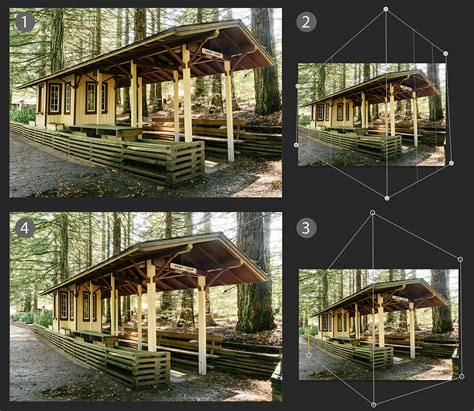
\includegraphics[width=1.0\textwidth]{images/Perspective Warp example.jpg}
	\end{center}
\end{frame}

\subsection{Options}		
\begin{frame}
	\frametitle{Perspective Warp Options}
	\begin{outline}
		\1 
	\end{outline}
\end{frame}

\subsection{Resources}		
\begin{frame}
	\frametitle{Additional Resources for the Perspective Warp}
	\begin{outline}
		\1 
		\2 
		\2
	\end{outline}
\end{frame}

\section{Puppet Warp}

\subsection{Puppet Warp}		

\begin{frame}
	\frametitle{Puppet Warp}
	\begin{outline}
		\1 
	\end{outline}
\end{frame}

	\begin{frame}
	\frametitle{How to use Puppet Warp}
	\begin{outline}
		\1 
	\end{outline}
\end{frame}

\subsection{Example}		
\begin{frame}
	\frametitle{Puppet Warp Example}
	\begin{center}
		\includegraphics[width=1.0\textwidth]{images/Puppet Warp example.png}
	\end{center}
\end{frame}

\subsection{Options}		
\begin{frame}
	\frametitle{Puppet Warp Options}
	\begin{outline}
		\1 
	\end{outline}
\end{frame}

\subsection{Resources}		
\begin{frame}
	\frametitle{Additional Resources for the Puppet Warp}
	\begin{outline}
		\1 How To Use Puppet Warp in Photoshop – Puppet Warp Guide
		\2  By:  Photoshop Training Channel
		\2 https://photoshoptrainingchannel.com/puppet-warp-in-photoshop/
		\1 Photoshop Puppet Warp 101: Everything You Wanted To Know
		\2  By:  Photoshop Training Channel
		\2 https://youtu.be/xRGt7byhS50
	\end{outline}
\end{frame}
	
\end{document}